\section{Laboratory work implementation}

\subsection{Tasks and Points}

\begin{enumerate}

\item Create a Windows application what will display a dialog box on some event (ex. on clicking some button)
\item Add a system menu to your application with at least 3 items (add actions to that items)
\item Hook keyboard input. Add 2 custom events for 2 different keyboard combinations (ex. change window background on ctrl+space)
\item Add a scroll bar that will change any visible parameter of any other element (color of a text) OR other 2 scroll bars that will manage main window size or position
\item Customize your application by adding an icon and using different cursor in application
\item Add a listbox and attach some events when any element is accessed (clicked)

\end{enumerate}
\subsection{Laboratory work analysis}

Link to my GitHub repository : 

\url{https://github.com/Tolea86/WP_ANDROID/tree/master/LAB_2/PW_LAB2}\\

My application has following features : it has two buttons centered in the middle of the application, on clicking one of these buttons open a dialog another one hooks keyboard input, pressing key "S" will show a loading dialog for one second, pressing key "R" will show a dialog, it also has a custom menu with 3 buttons, one is always visible and clicking on it will display a message into a dialog, other 2 are hidden and one of them click will destroy the center button which opens a dialog, but another one will change the color of the background into one random color. It also has two lists on top and bottom of the view with randomly generated colors, clicking on a element from the top will change the color of the text centered in the view, clicking on an element from the bottom will change the background color of one randomly chosen button from the center.

\subsection{Prove your work with screens}

a)

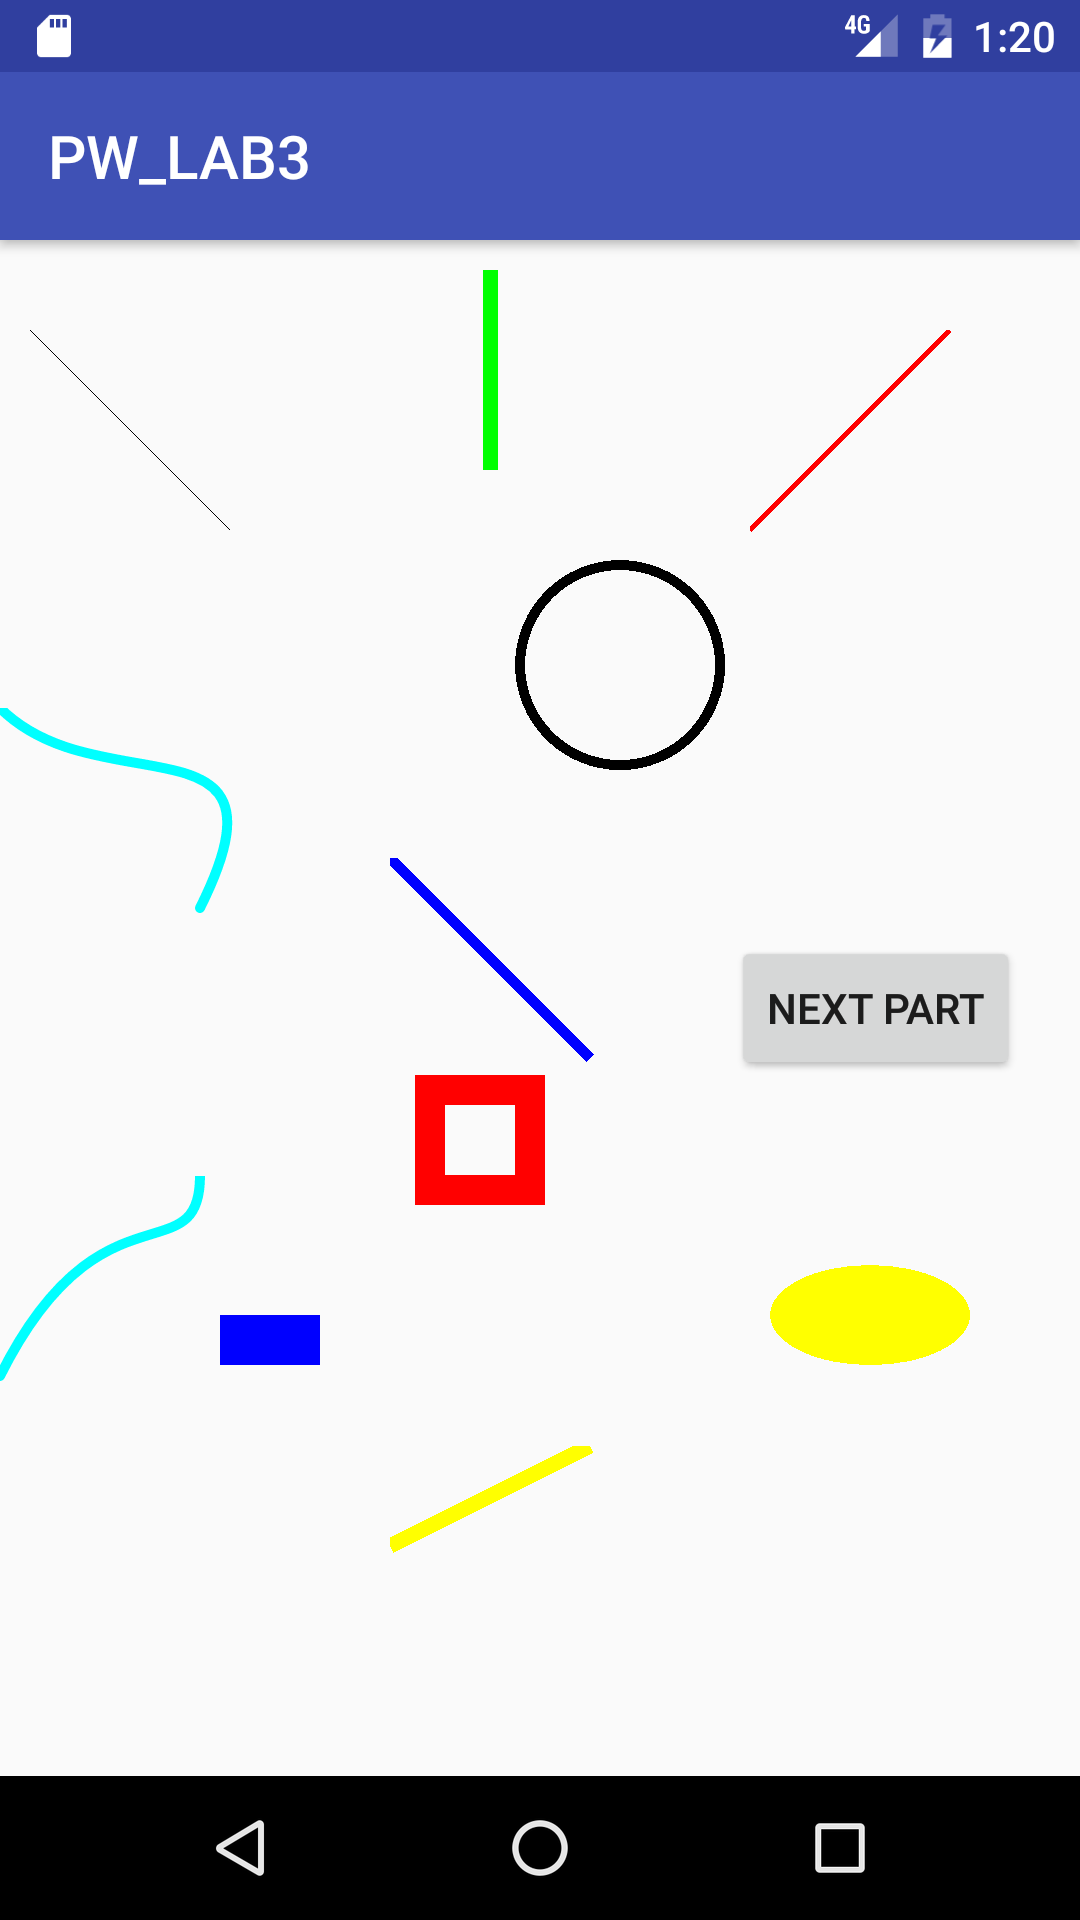
\includegraphics[scale=0.2]{screen1}
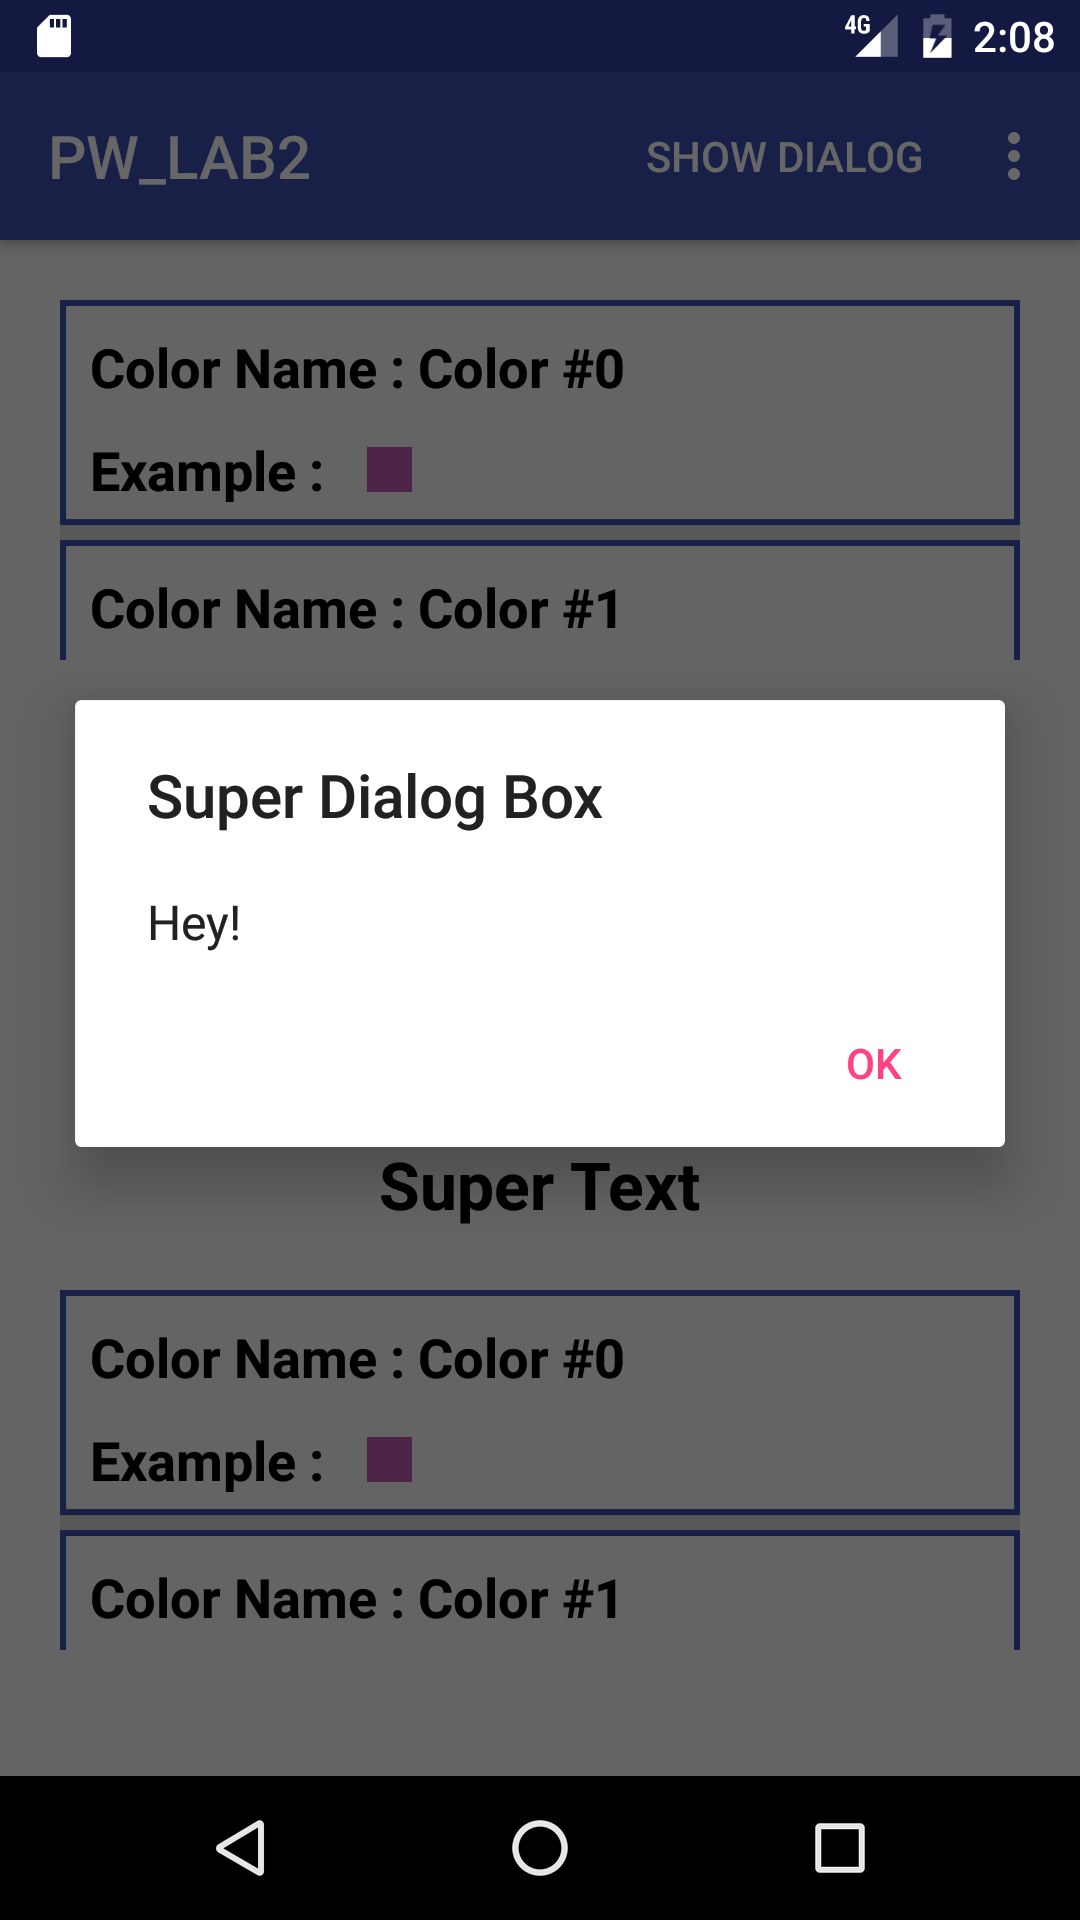
\includegraphics[scale=0.2]{screen2}

b)

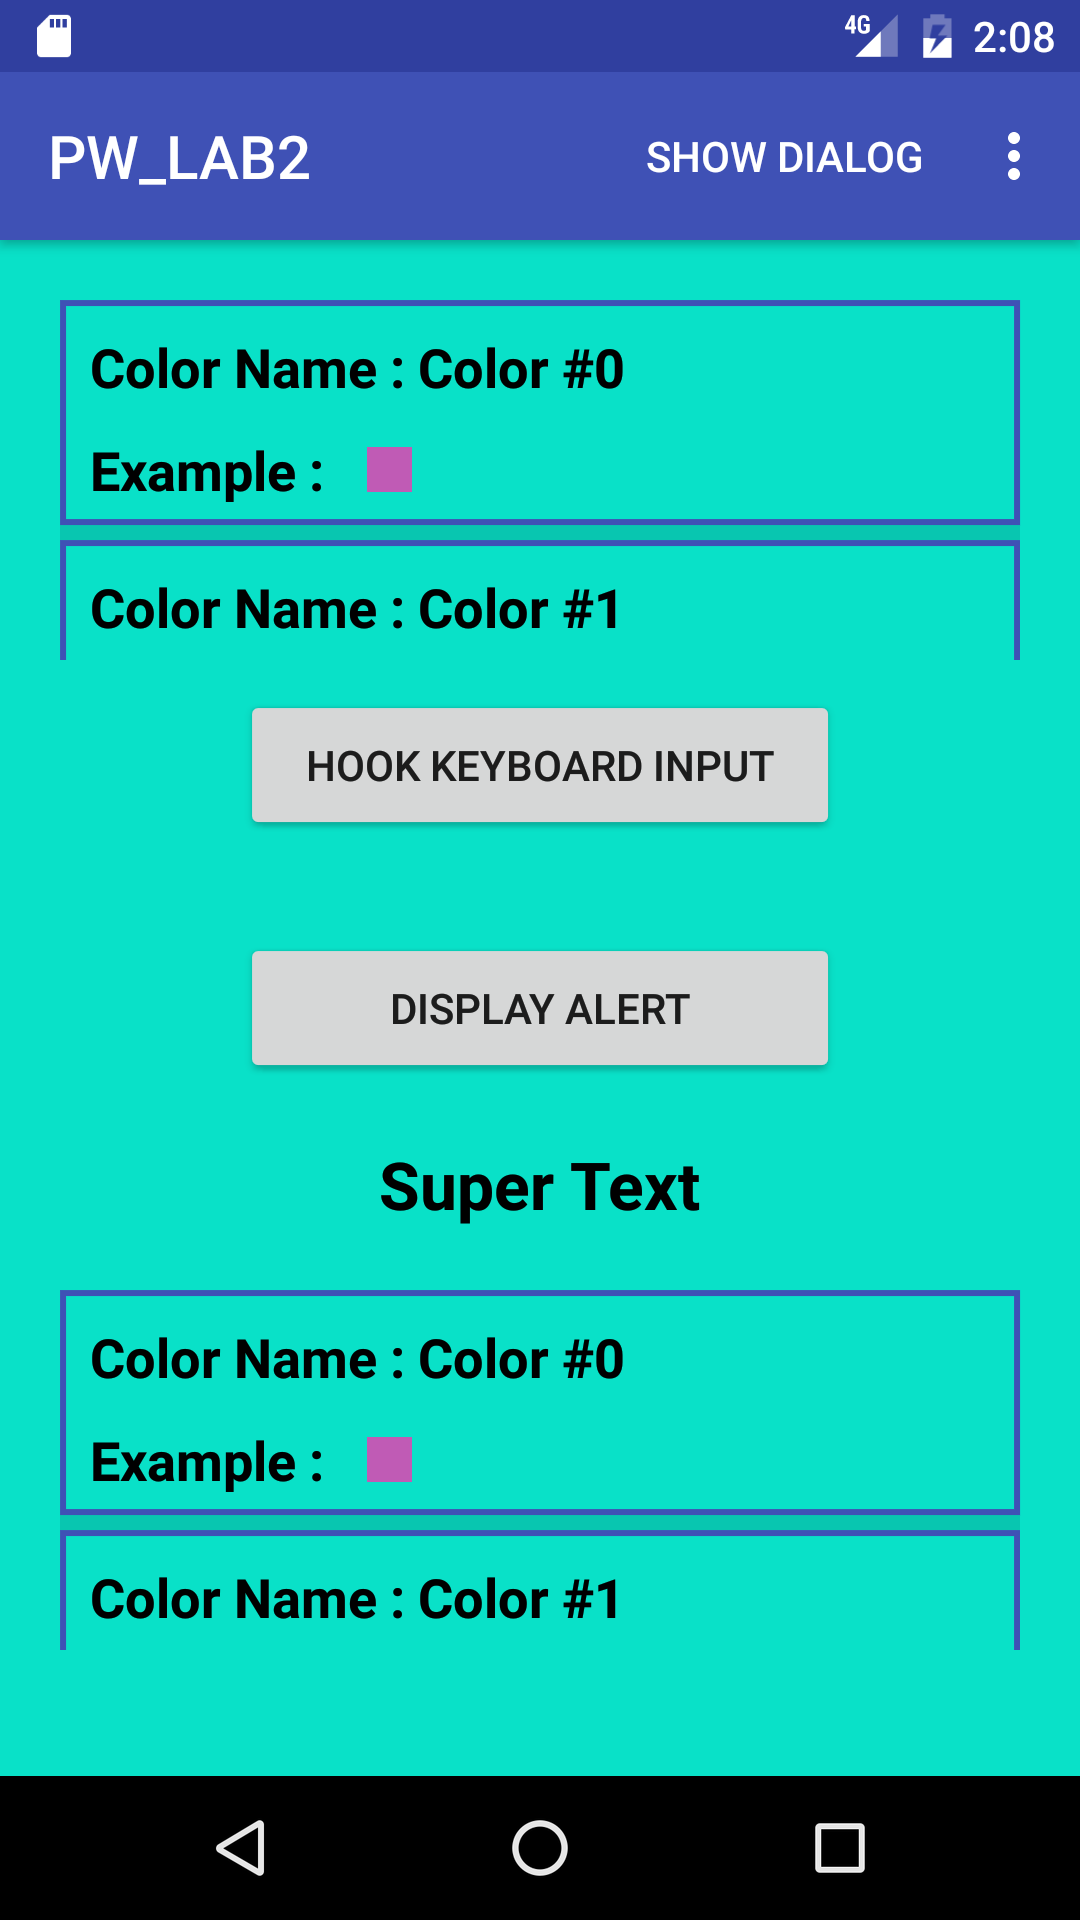
\includegraphics[scale=0.2]{screen3}
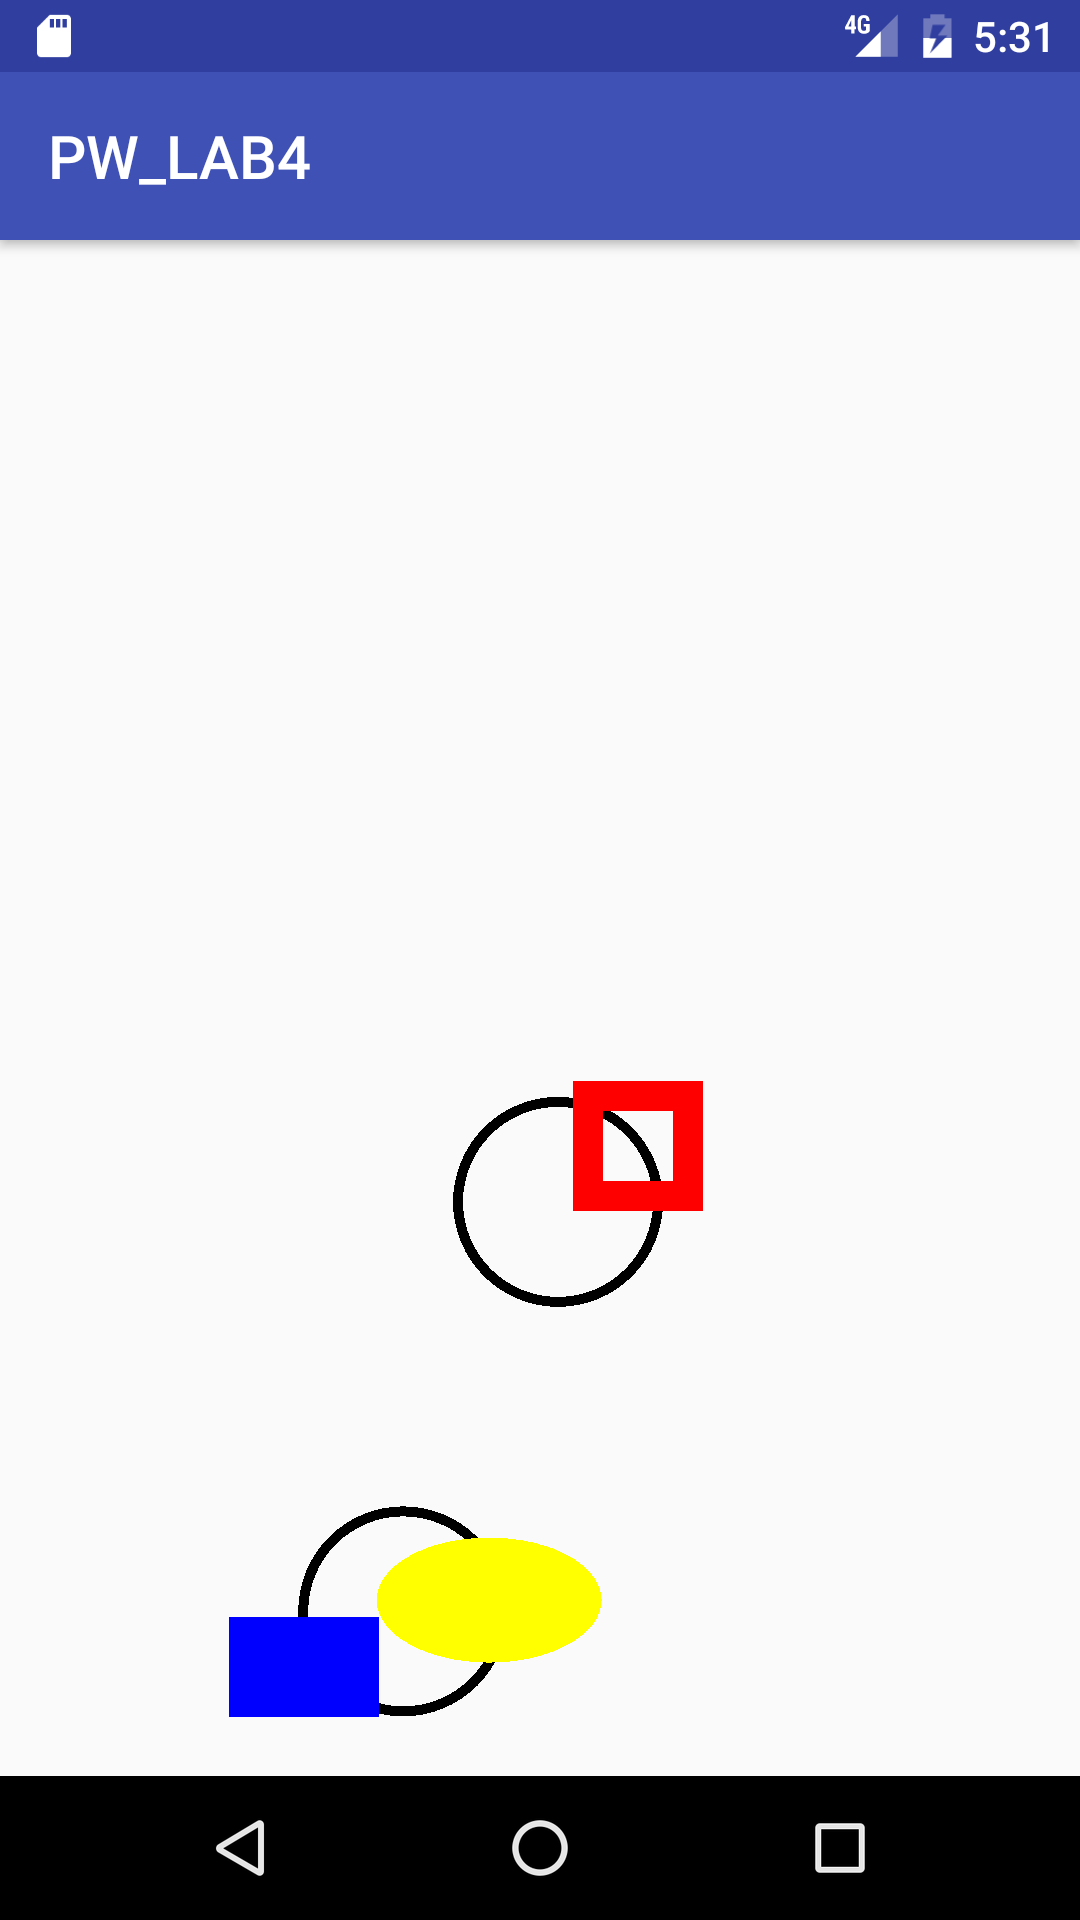
\includegraphics[scale=0.2]{screen4}

c)

"S" clicked

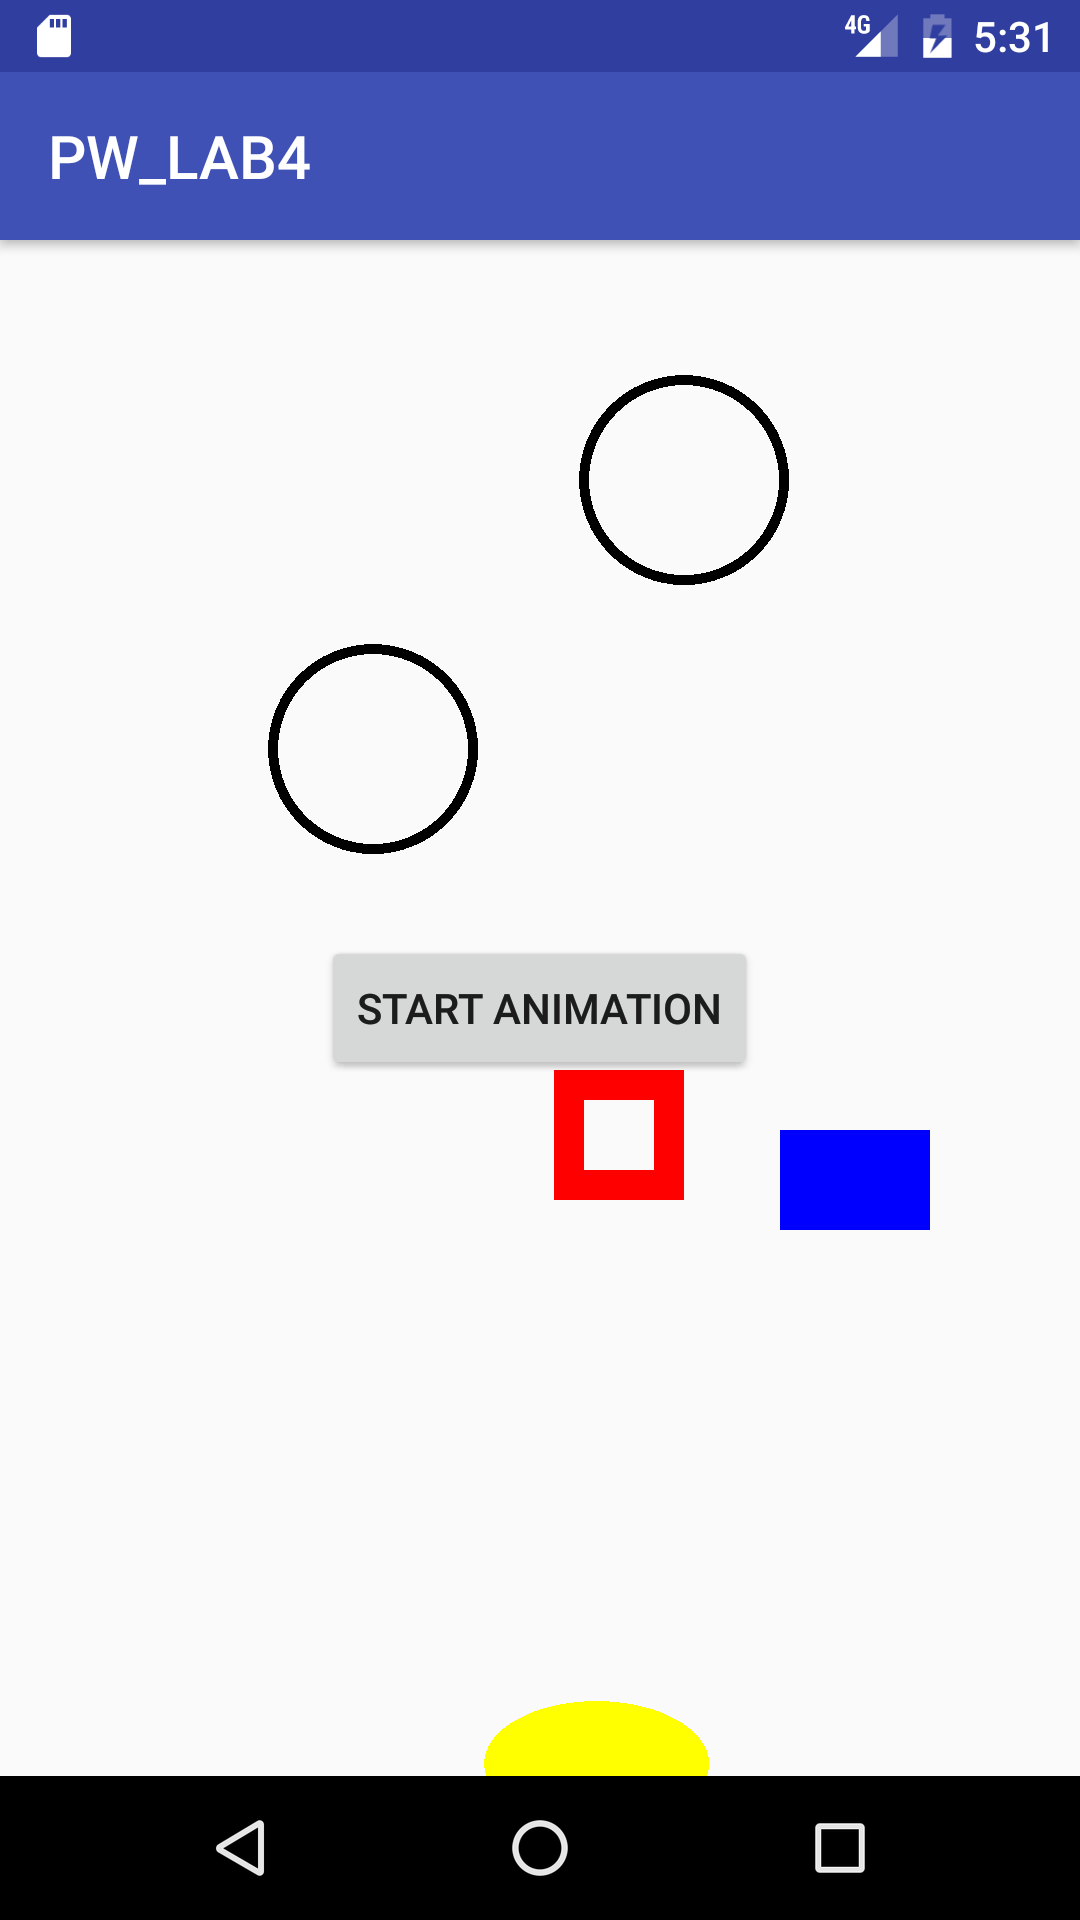
\includegraphics[scale=0.2]{screen5}

"R"clicked 

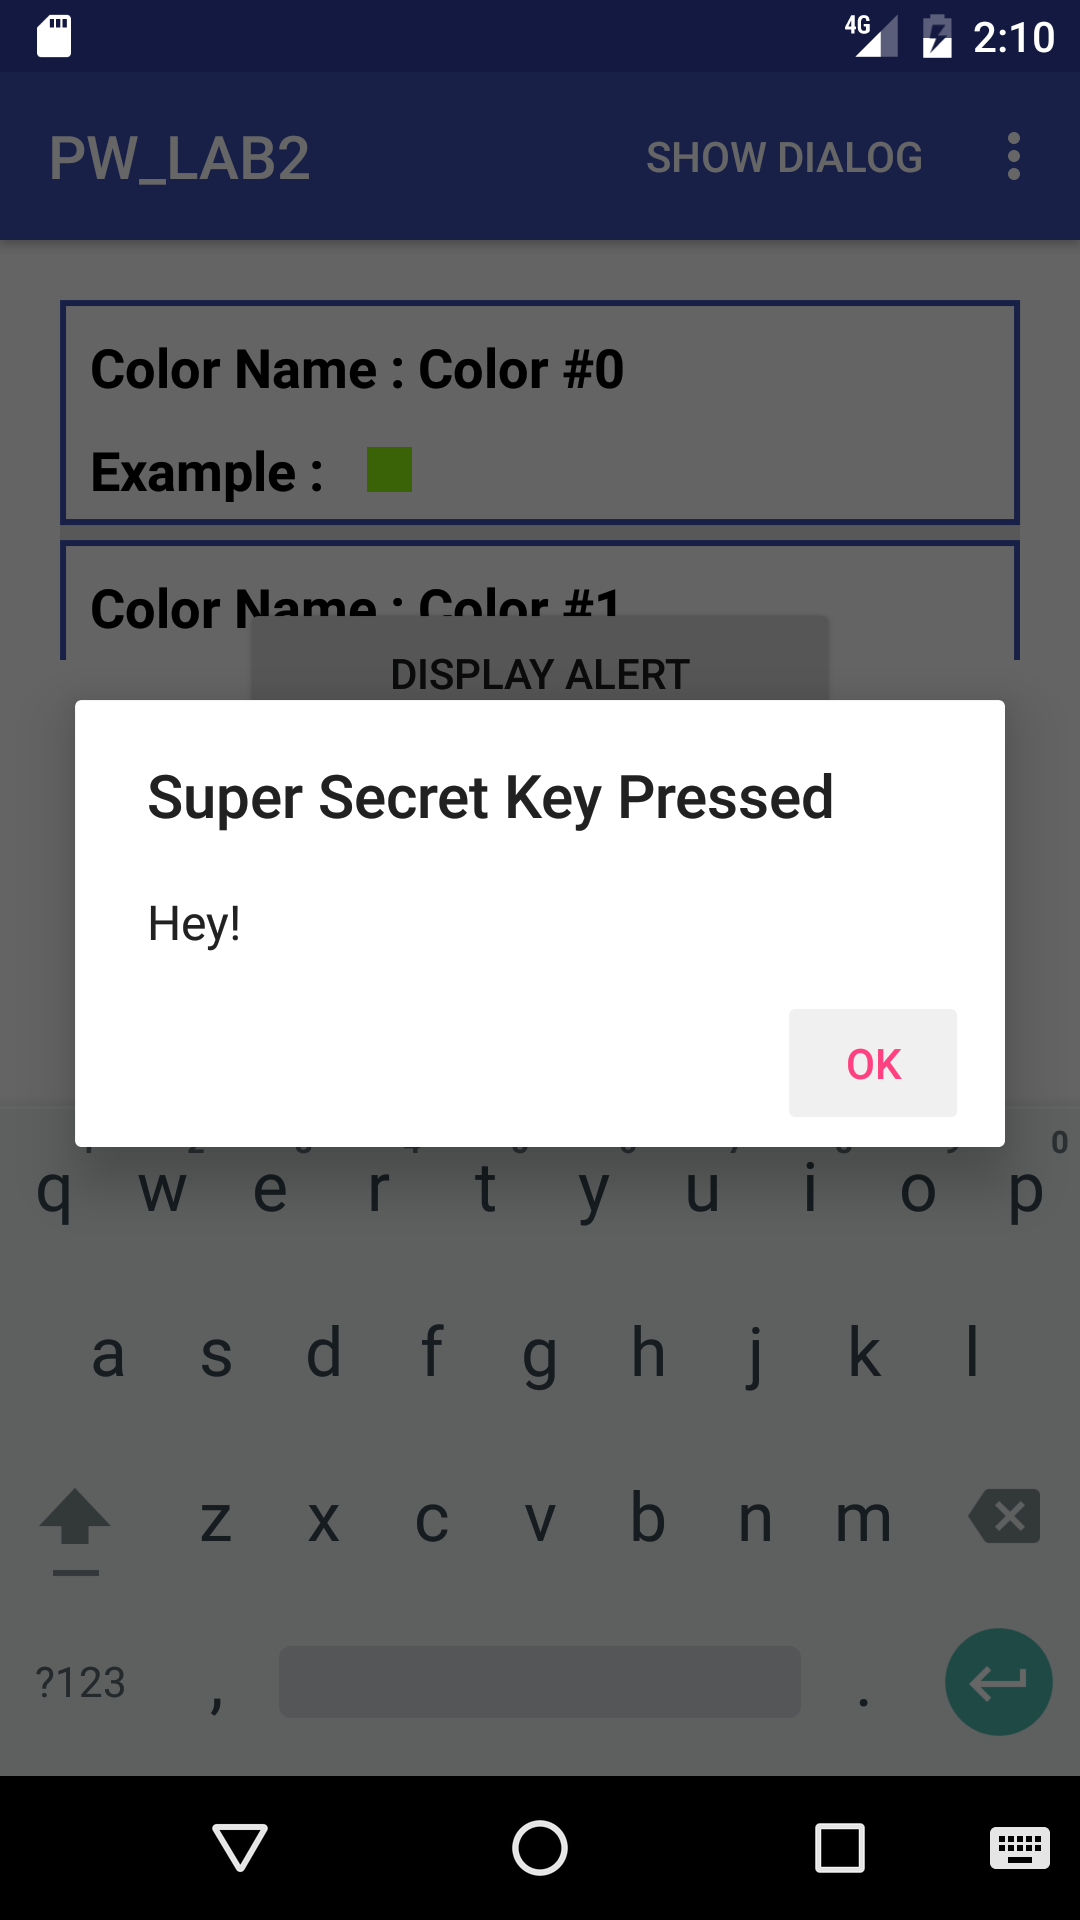
\includegraphics[scale=0.2]{screen6}

d) Top list with scroll bar

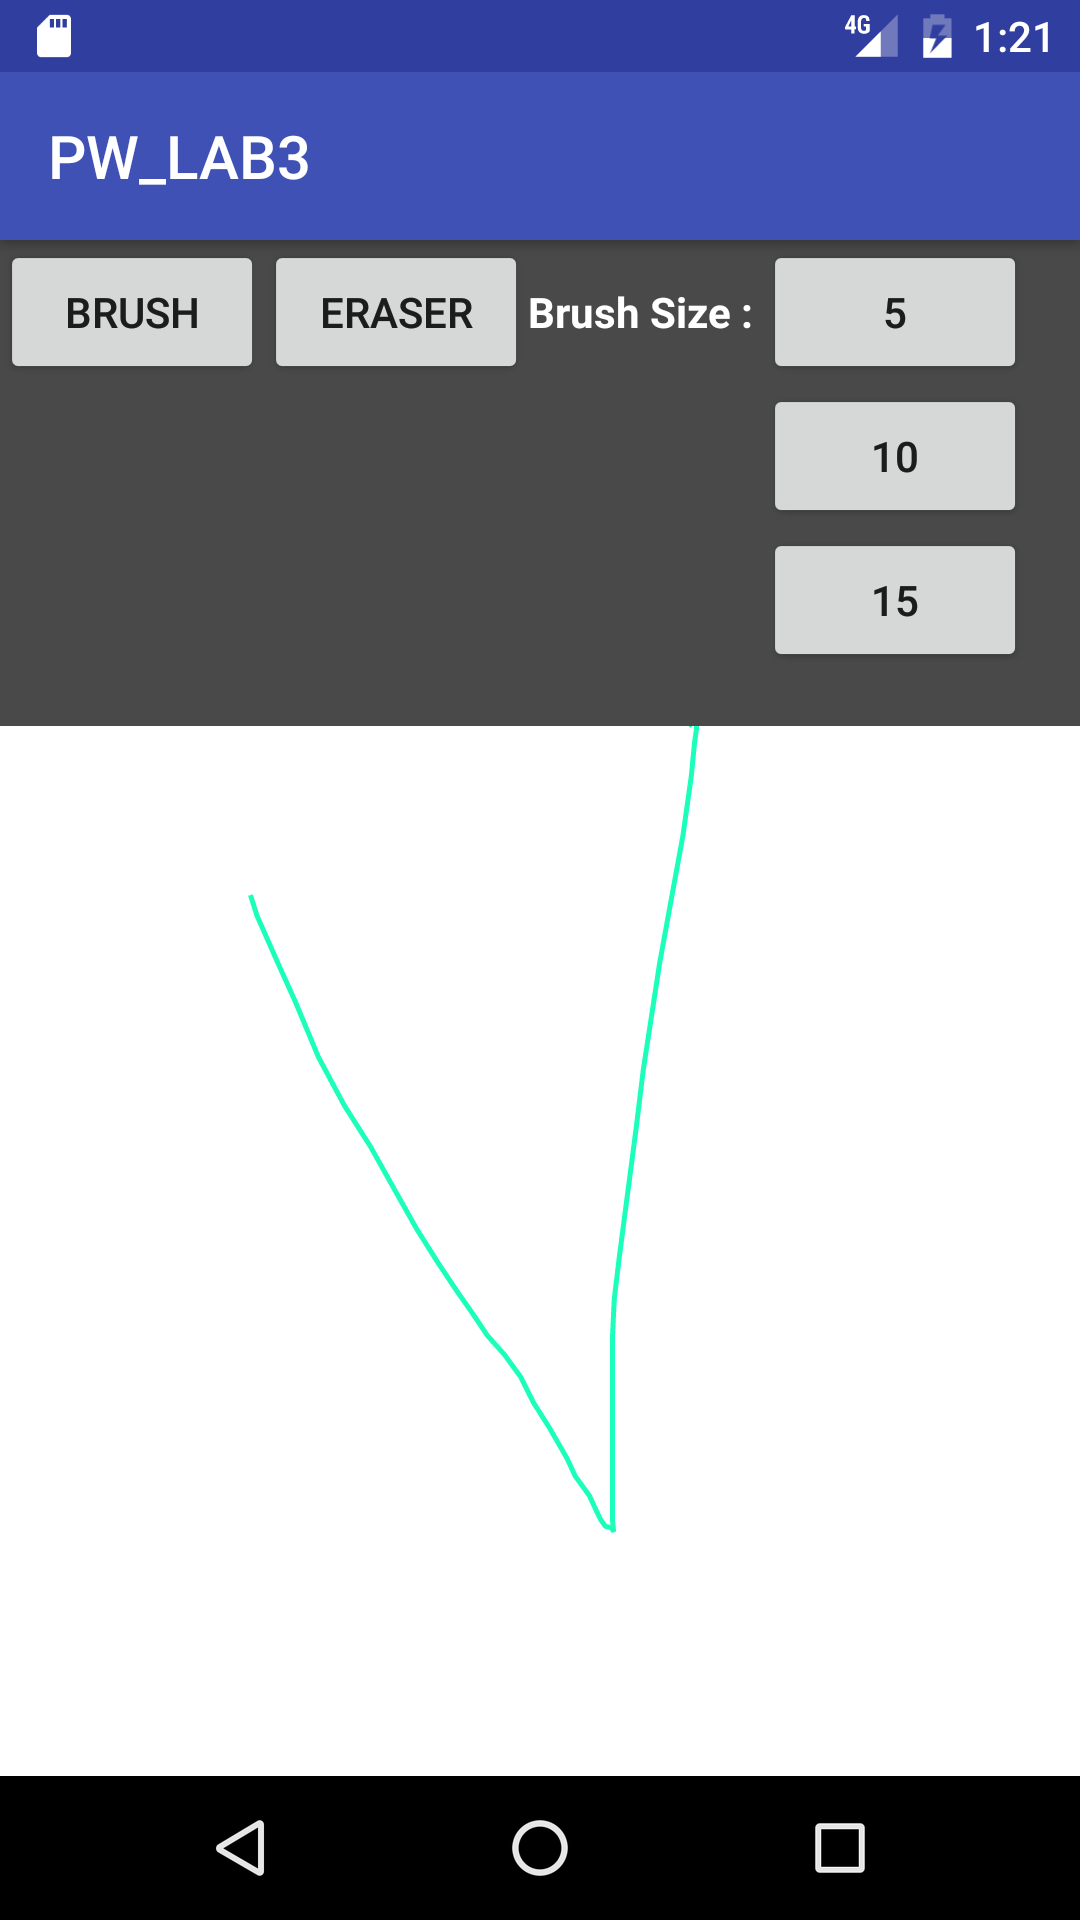
\includegraphics[scale=0.2]{screen7}

e)

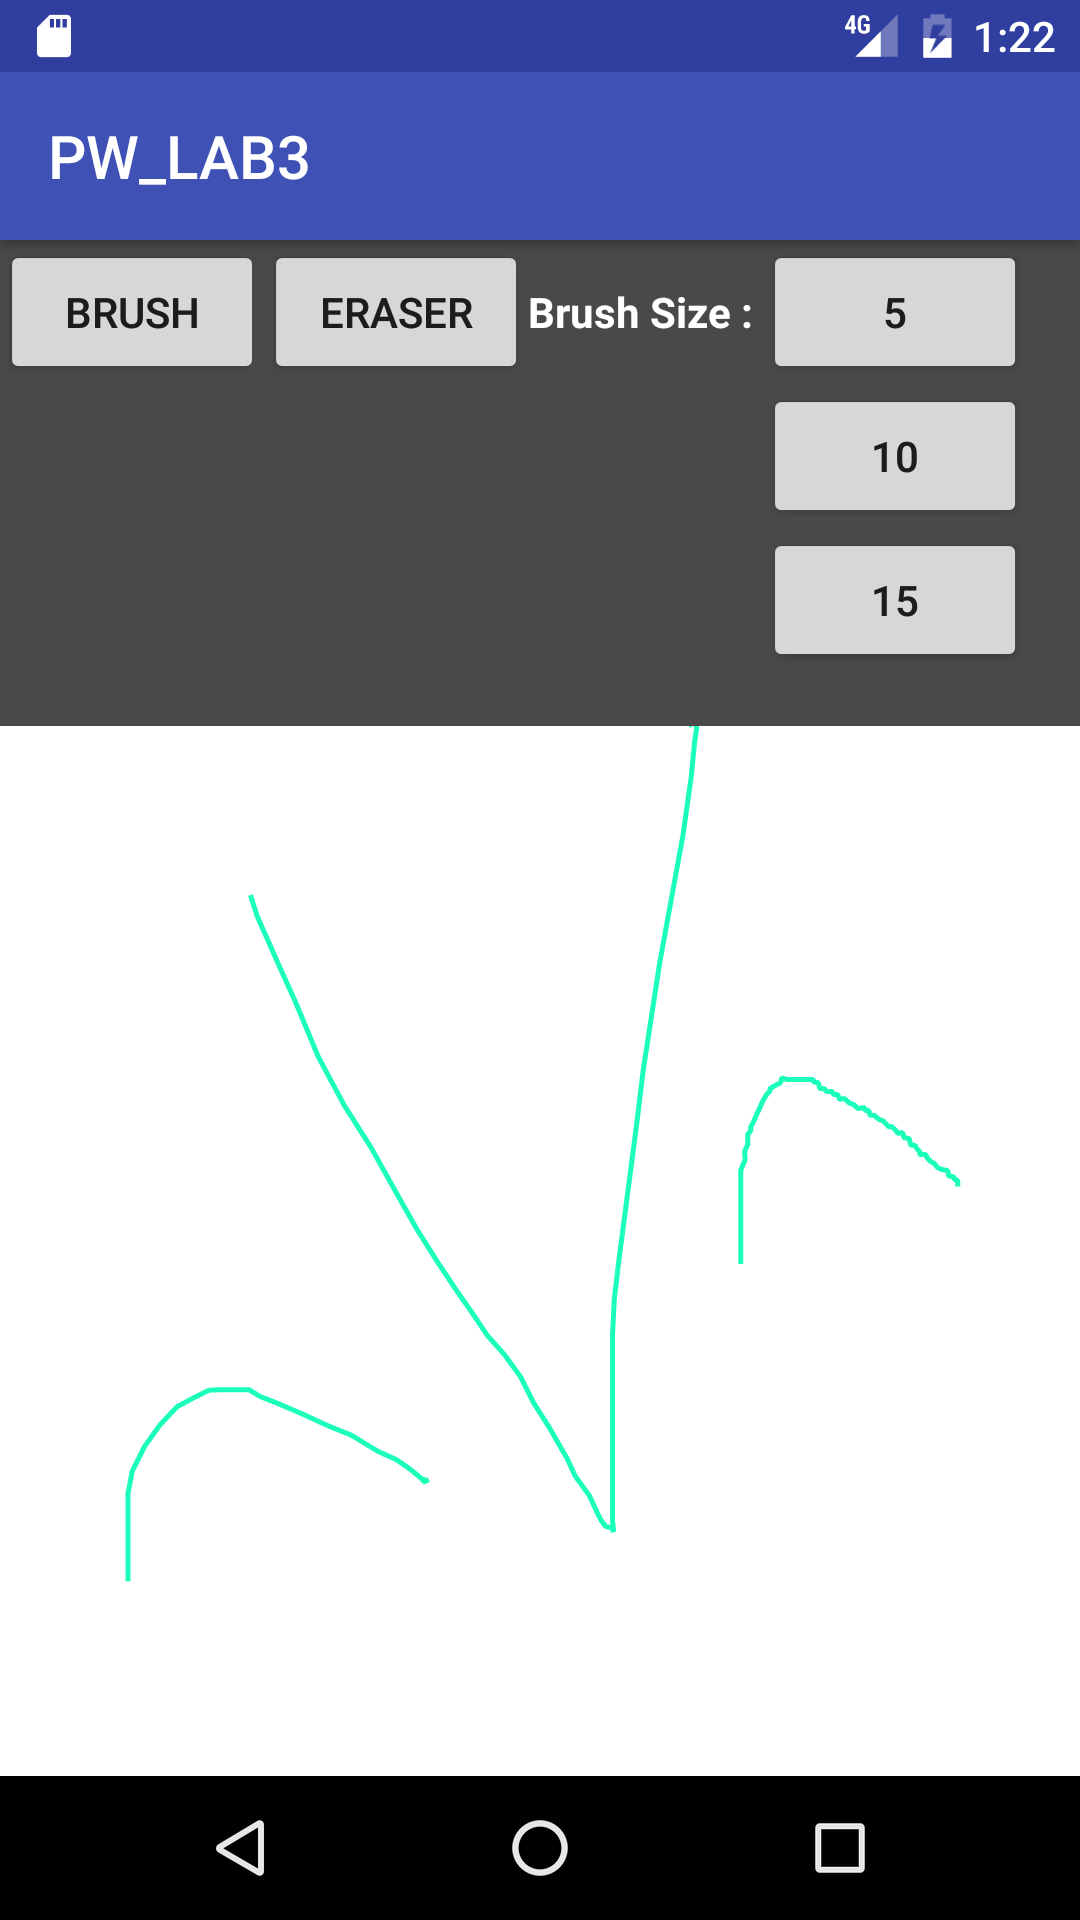
\includegraphics[scale=0.2]{screen8}

f) Bottom list with random action

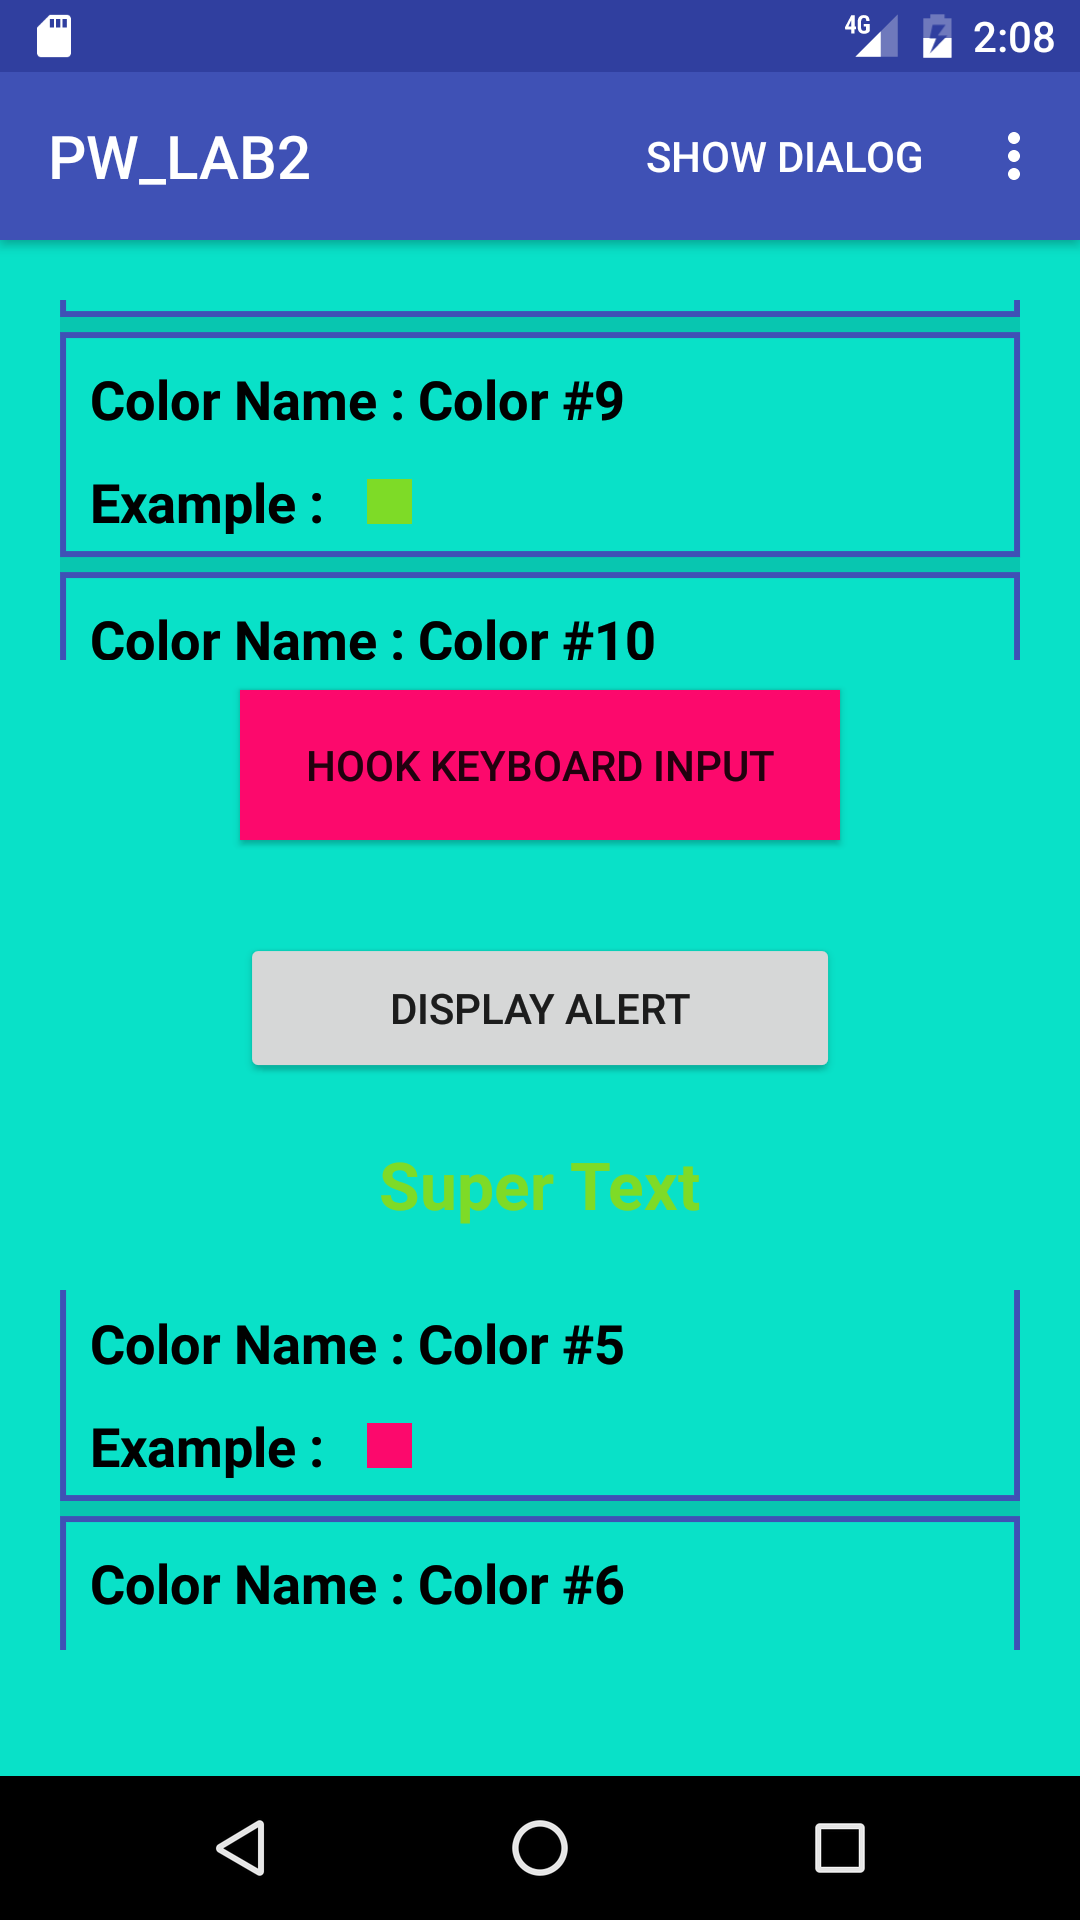
\includegraphics[scale=0.2]{screen9}

\clearpage